% Chapter 3

\chapter{Results} % Main chapter title

\label{Results} % For referencing the chapter elsewhere, use \ref{Chapter1} 

\lhead{Chapter 3. \emph{Results}} % This is for the header on each page - perhaps a shortened title

\section{Results}

\clearpage
\subsection{Fitness Based Search}

\begin{figure}[h!]
\centering
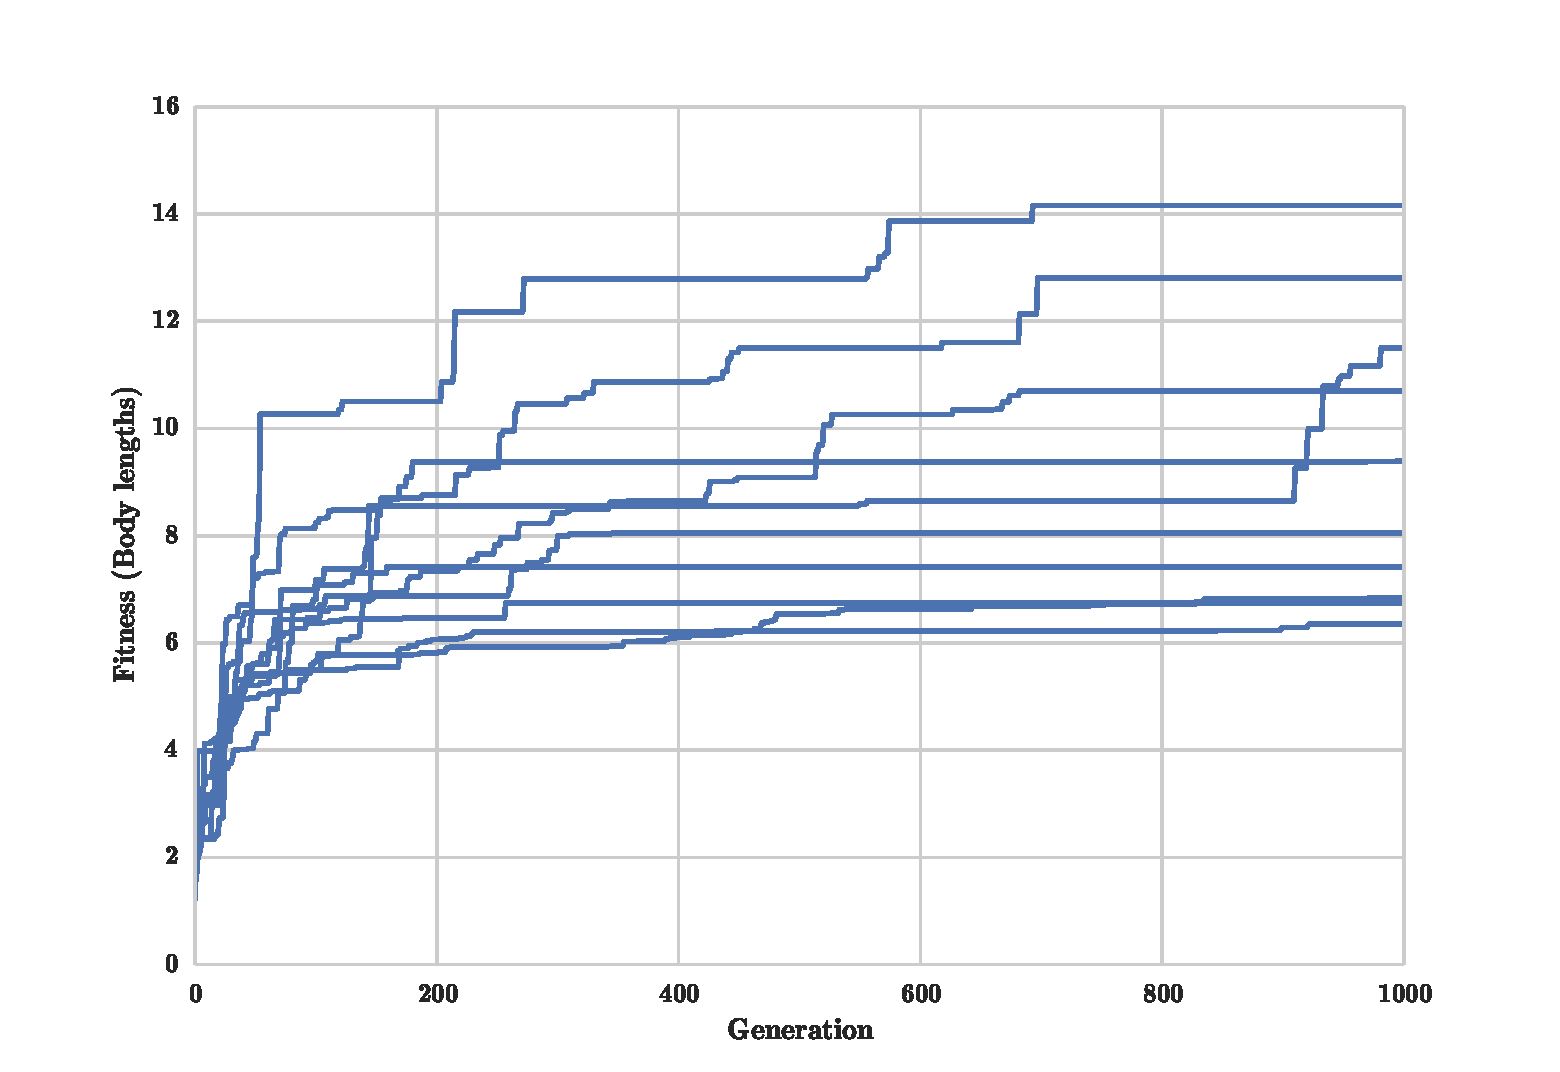
\includegraphics[width=1.0\textwidth]{Figures/Results/indRunsSize10Fitness.pdf}
\caption{Caption}
\caption{Best so far fitness in body lengths displacement of softbot's center of mass from $10$ runs for fitness based search. The gravity acceleration for this experiment used was $-27.468\   m/s^2$, the size of the lattice $10\times 10\times10$ and $4$ available materials ($2$-actuated).}
\end{figure}

\begin{figure}[h!]
\centering
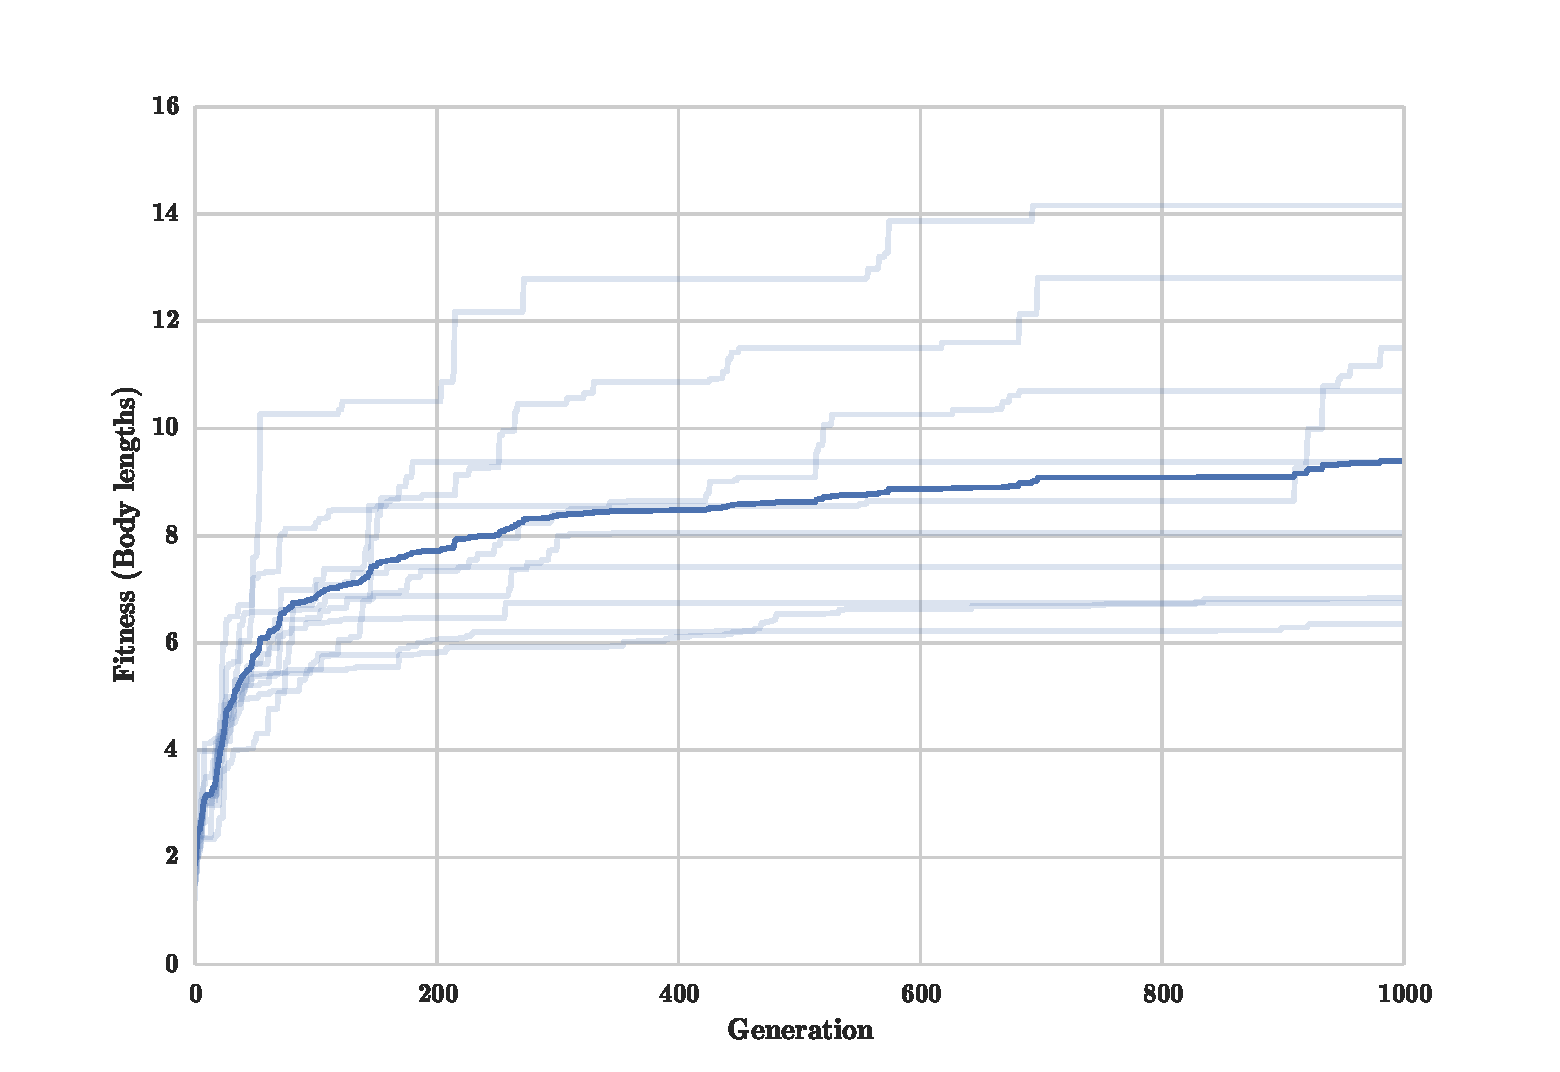
\includegraphics[width=1.0\textwidth]{Figures/Results/indRunsAvgSize10Fitness.pdf}
\caption{Best so far fitness in body lengths displacement of softbot's center of mass from $10$ runs together with their mean (thick line) for fitness based search. The gravity acceleration for this experiment used was $-27.468\   m/s^2$, the size of the lattice $10\times 10\times10$ and $4$ available materials ($2$-actuated).}
\label{fig:indRunsAvgSize10Fitness}
\end{figure}















\clearpage
\subsection{Novelty Search}

\begin{figure}[h!]
\centering
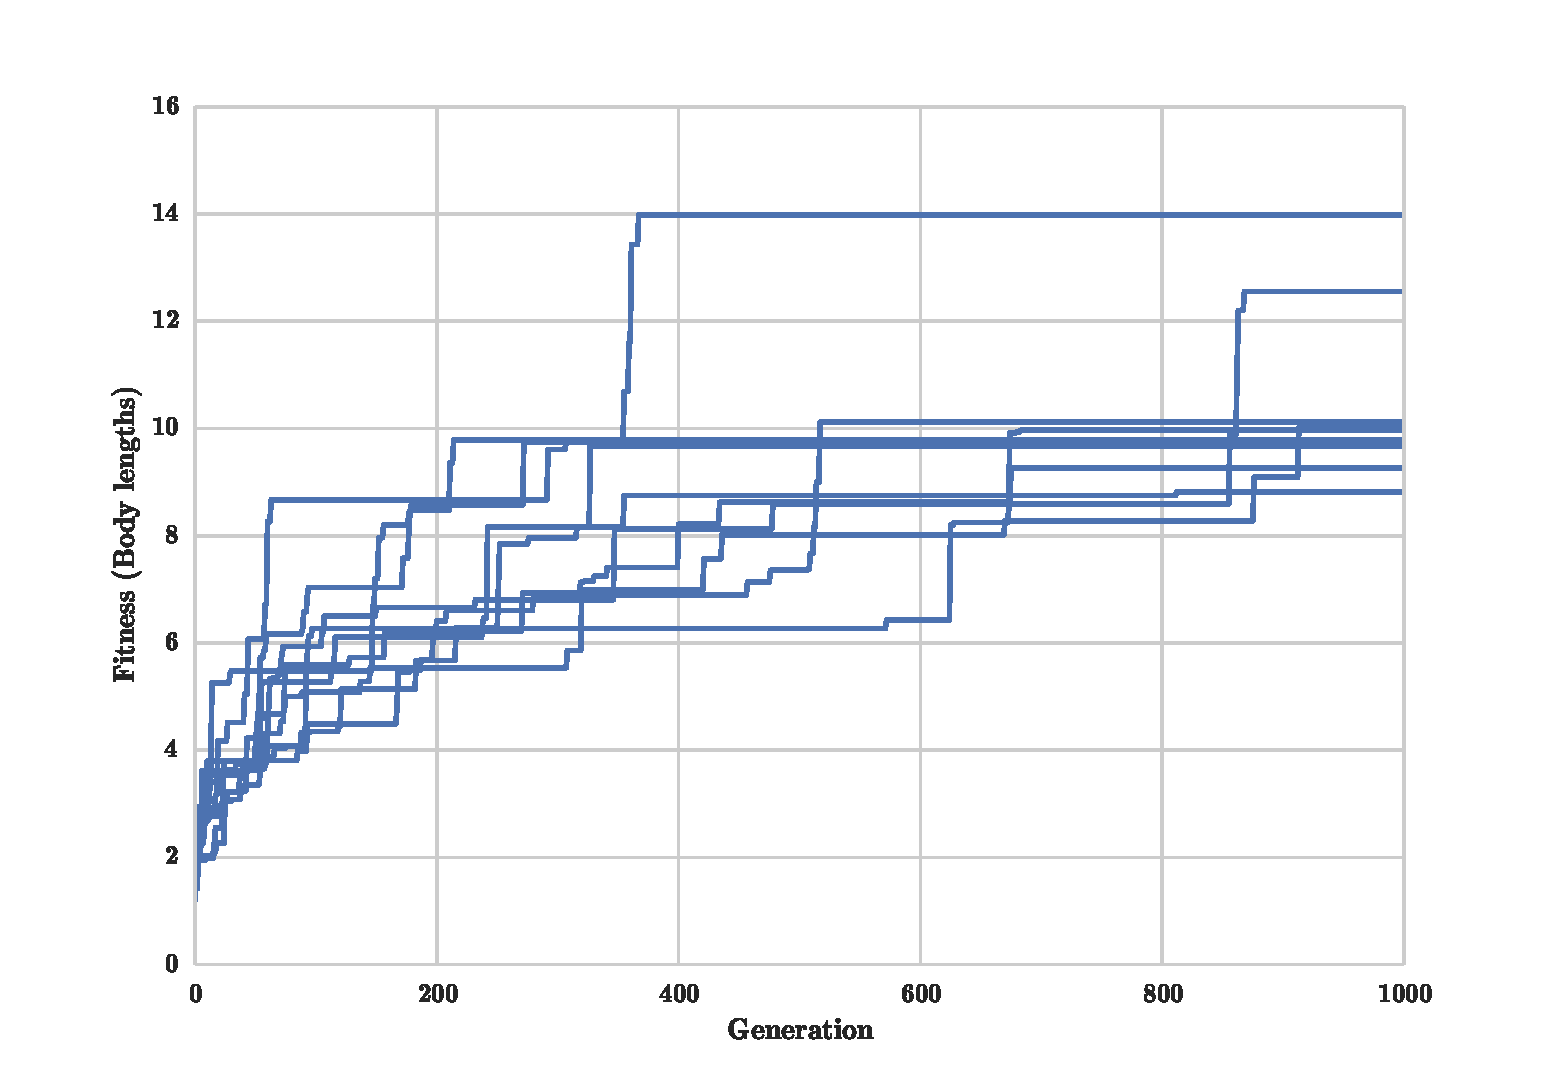
\includegraphics[width=1.0\textwidth]{Figures/Results/indRunsSize10Novelty.pdf}
\caption{Best so far fitness in body lengths displacement of softbot's center of mass from $10$ runs for novelty search. The gravity acceleration for this experiment used was $-27.468\   m/s^2$, the size of the lattice $10\times 10\times10$ and $4$ available materials ($2$-actuated).}
\label{fig:indRunsSize10Novelty}
\end{figure}

\begin{figure}[h!]
\centering
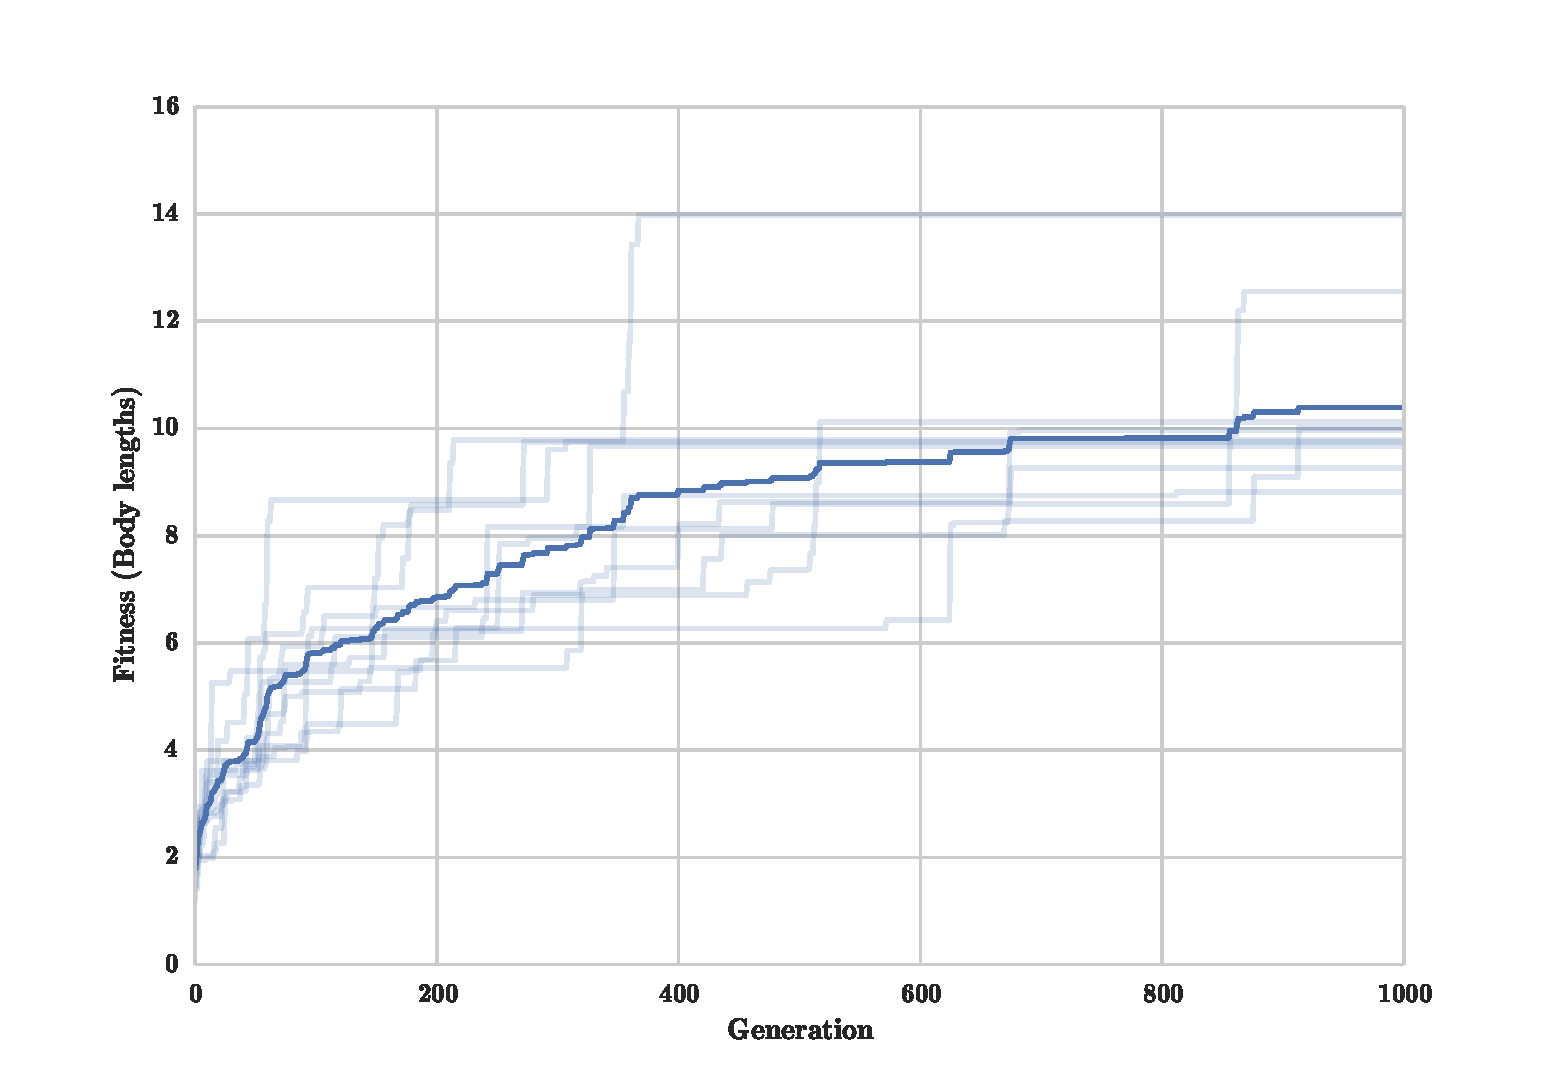
\includegraphics[width=1.0\textwidth]{Figures/Results/indRunnAvgSize10Novelty.pdf}
\caption{Best so far fitness in body lengths displacement of softbot's center of mass from $10$ runs together with their mean (thick line) for novelty search. The gravity acceleration for this experiment used was $-27.468\   m/s^2$, the size of the lattice $10\times 10\times10$ and $4$ available materials ($2$-actuated).}
\label{fig:indRunnAvgSize10Novelty}
\end{figure}


\begin{figure}
\centering
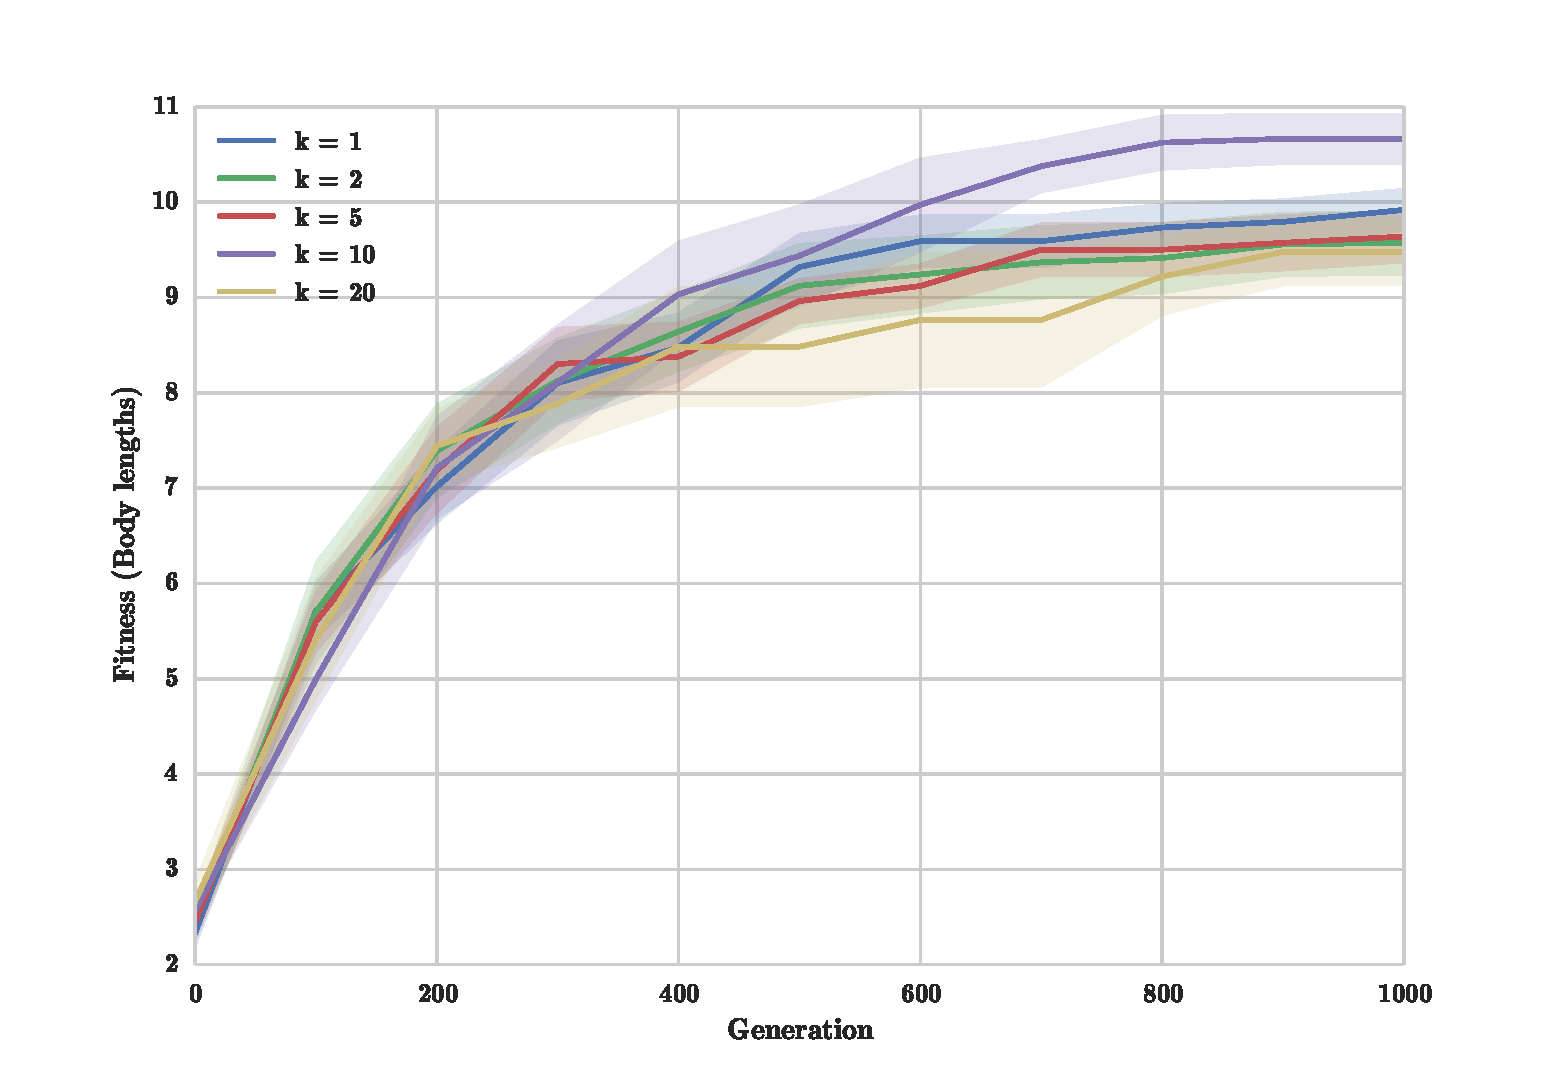
\includegraphics[width=1.0\textwidth]{Figures/Results/KnnExperimentSize5.pdf}
\caption{Novelty search - best so far fitness in body lengths displacement of softbot's center of mass from $10$ runs together with their mean (thick line). The novelty is computed as the average distance from the $K$-nearest behaviors for $K \in \lbrace 1,2,5,10,20 \rbrace $. The gravity acceleration for this experiment used was $-27.468\   m/s^2$, the size of the lattice $5\times 5\times5$ and $4$ available materials ($2$-actuated).}
\label{fig:KnnExperimentSize5}
\end{figure}


















\clearpage
\subsection{Novelty-Fitness Based Search Comparison}

\begin{figure}[h!]
\centering
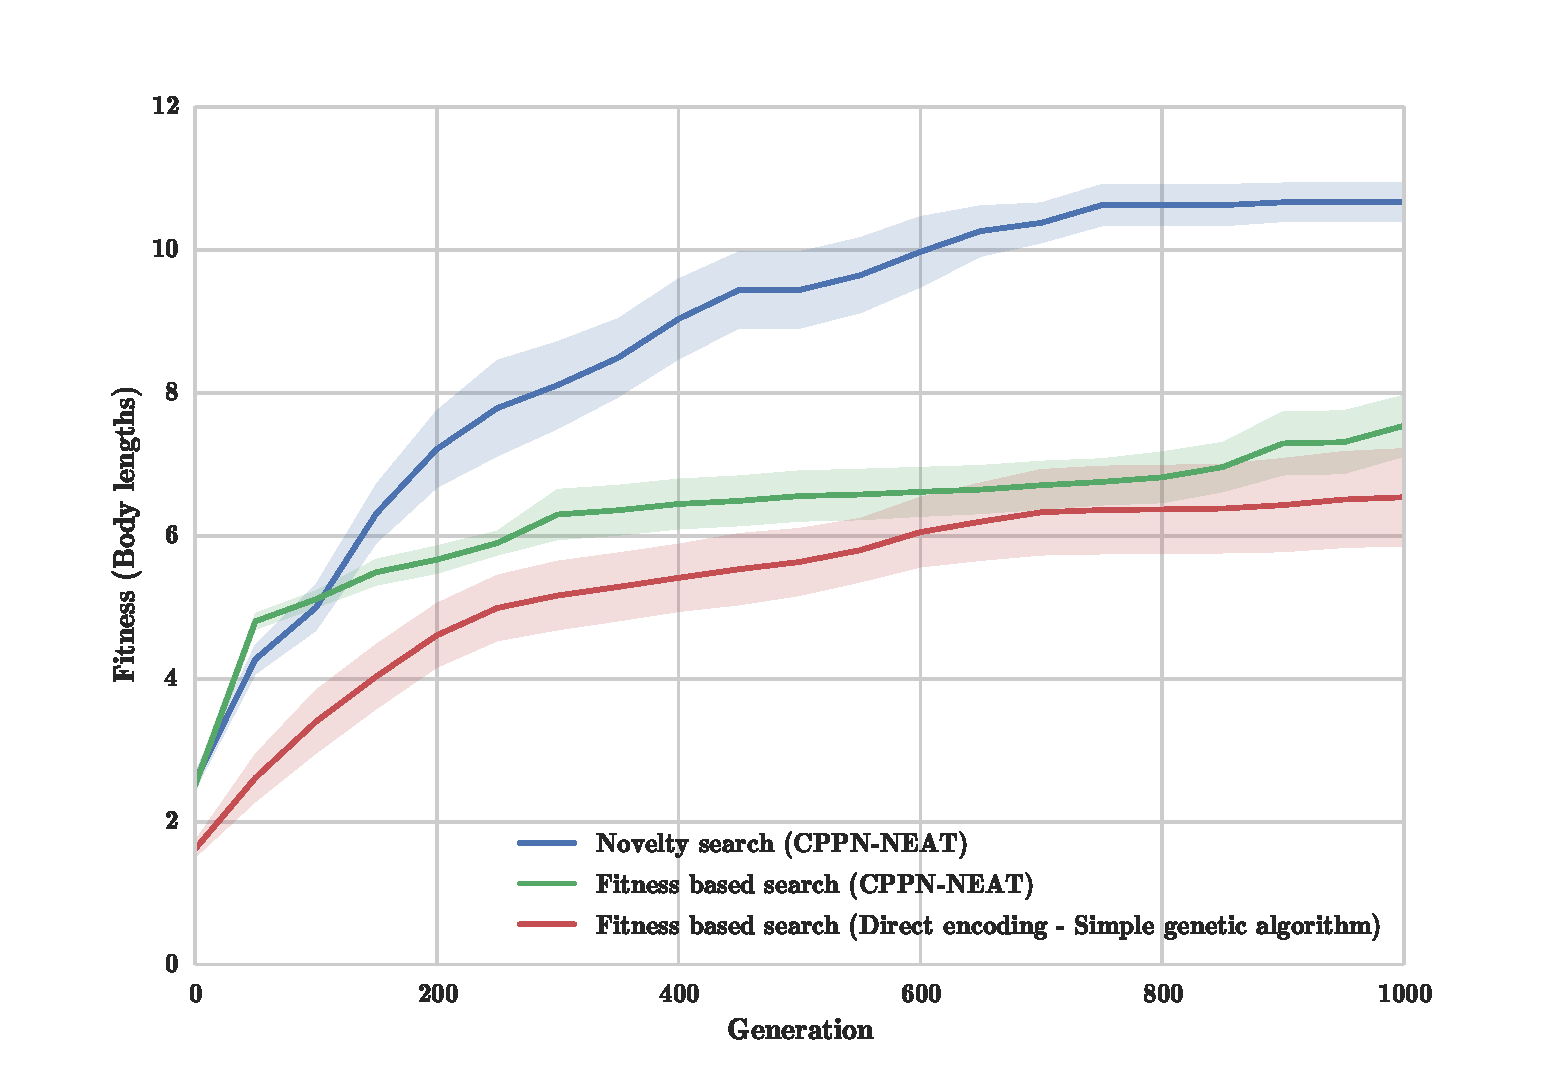
\includegraphics[width=1.0\textwidth]{Figures/Results/FitvsNovVsDirSize5.pdf}
\caption{Best so far fitness in body lengths displacement of softbot's center of mass averaged over $10$ runs together with the standard deviation error. The gravity acceleration for this experiment used was $-27.468\   m/s^2$, the size of the lattice $5\times 5\times5$ and $4$ available materials ($2$-actuated).}
\label{fig:FitvsNovVsDirSize5}
\end{figure}

\begin{figure}[h!]
\centering
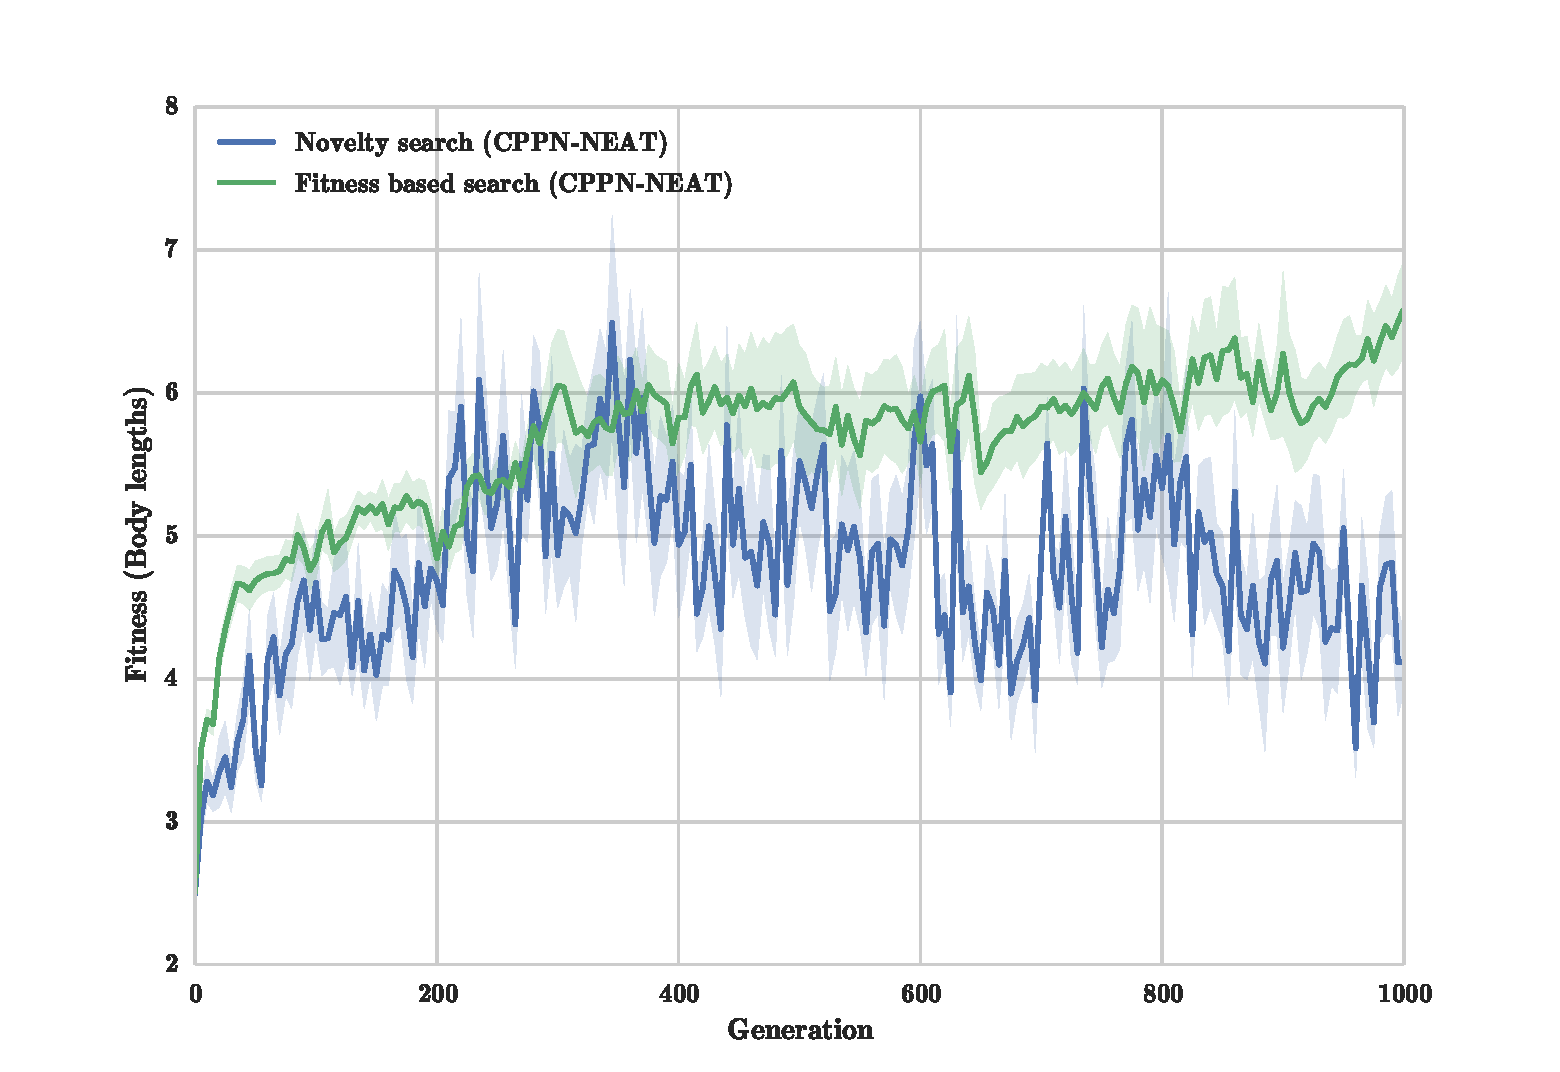
\includegraphics[width=1.0\textwidth]{Figures/Results/AvgGenerChampNoveltyFitnessSize5.pdf}
\caption{Fitness of the generation champion (best individual) per generation in body lengths displacement of softbot's center of mass averaged over $10$ runs together with the standard deviation error. The gravity acceleration for this experiment used was $-27.468\   m/s^2$, the size of the lattice $5\times 5\times5$ and $4$ available materials ($2$-actuated).}
\label{fig:AvgGenerChampNoveltyFitnessSize5}
\end{figure}

\begin{figure}[h!]
\centering
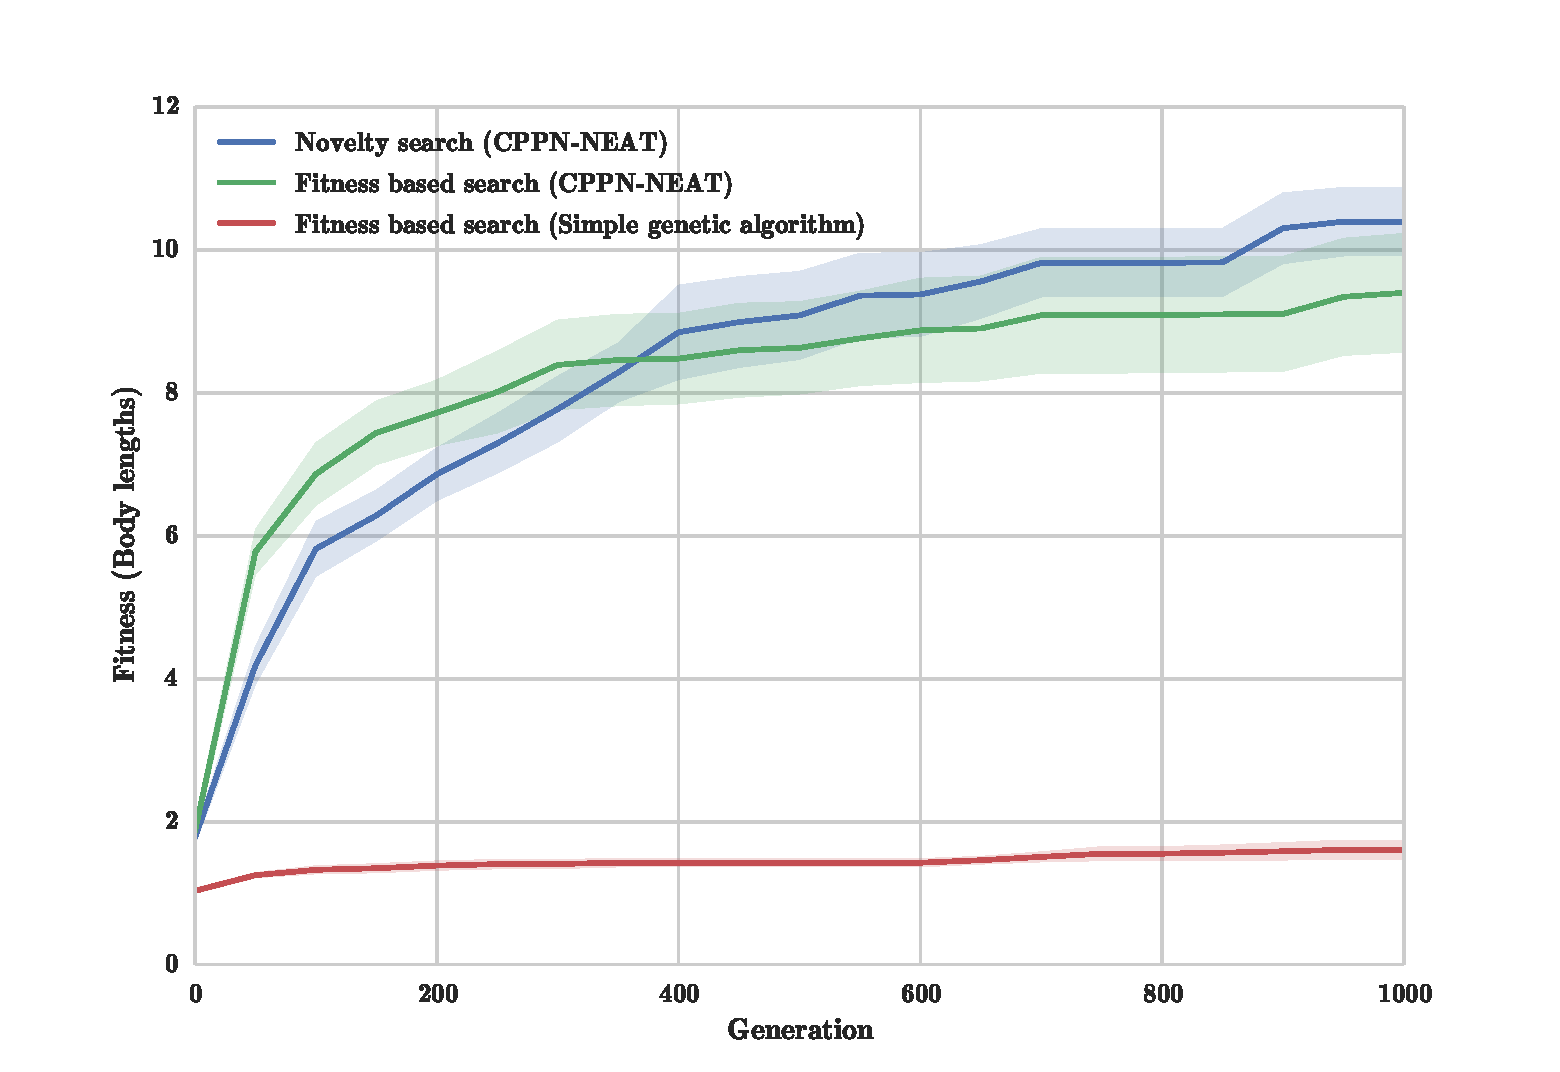
\includegraphics[width=1.0\textwidth]{Figures/Results/FitvsNovVsDirSize10.pdf}
\caption{Best so far fitness in body lengths displacement of softbot's center of mass averaged over $10$ runs together with the standard deviation error. The gravity acceleration for this experiment used was $-27.468\   m/s^2$, the size of the lattice $10\times 10\times10$ and $4$ available materials ($2$-actuated).}
\label{fig:FitvsNovVsDirSize10}
\end{figure}

\begin{figure}
\centering
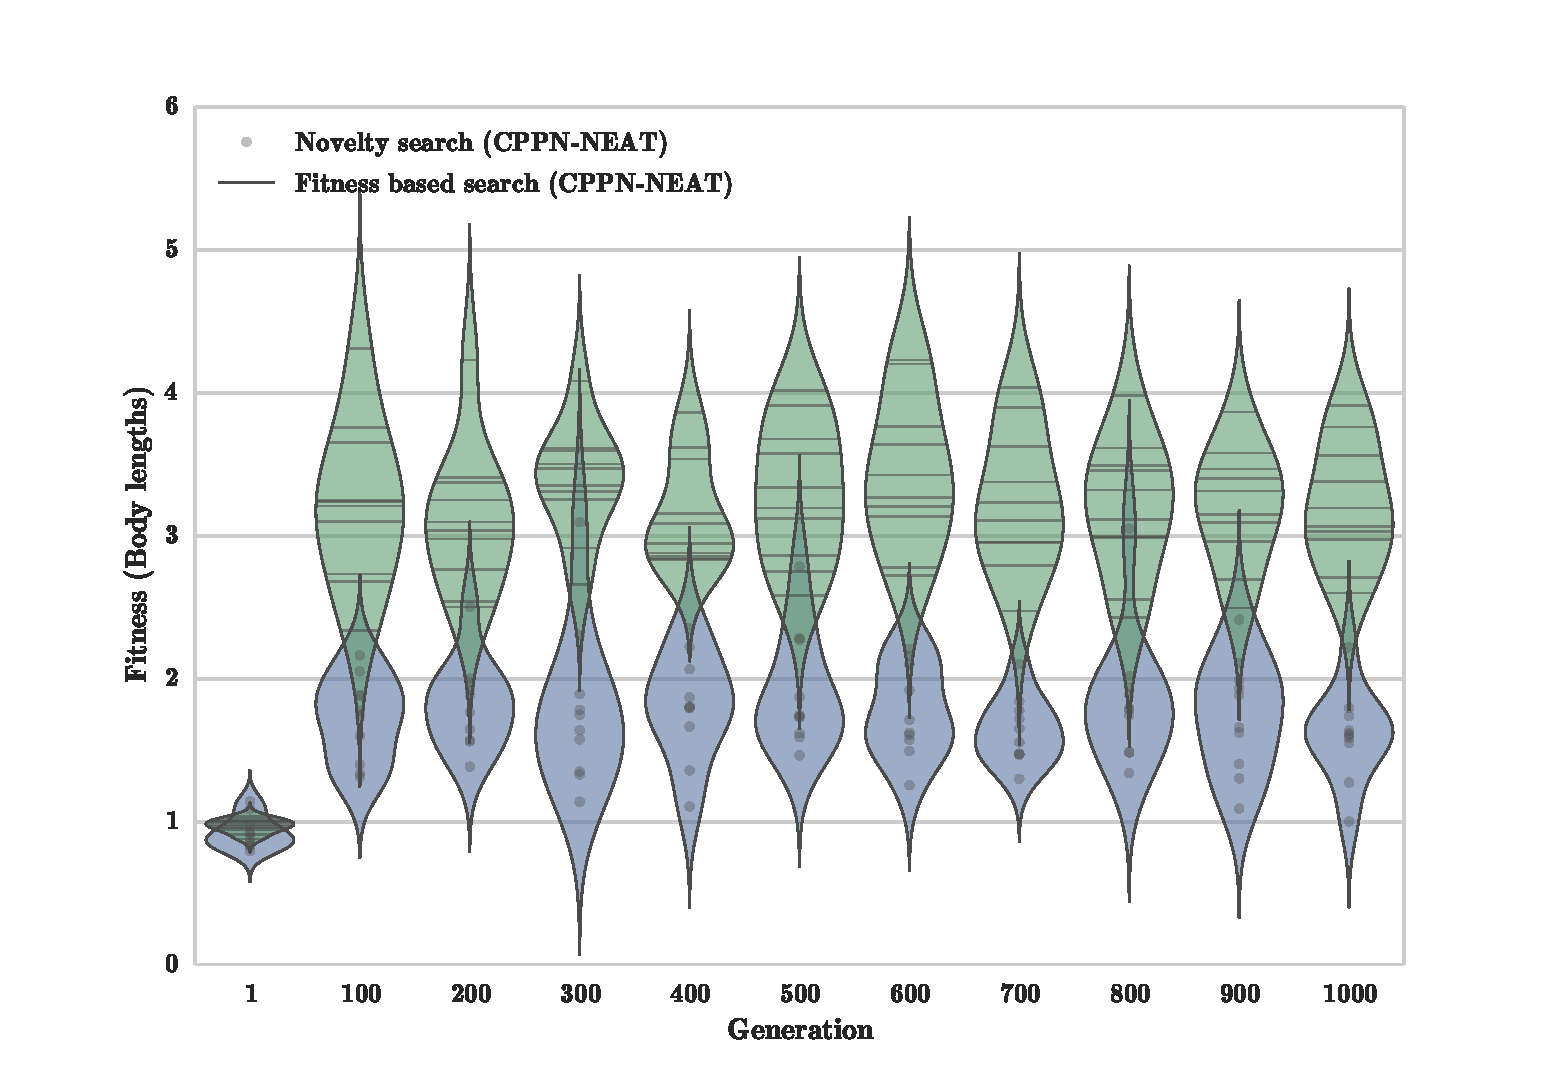
\includegraphics[width=1.0\textwidth]{Figures/Results/ViolinPlotsAvgGenFitSize5.pdf}
\caption{Distributions of average population fitness per generation over 10 runs. The gravity acceleration for this experiment used was $-27.468\   m/s^2$, the size of the lattice $5\times 5\times5$ and $4$ available materials ($2$-actuated). Blue (Novelty search), Green(Fitness based search).}
\label{fig:ViolinPlotsAvgGenFitSize5}
\end{figure}


\begin{figure}
\centering
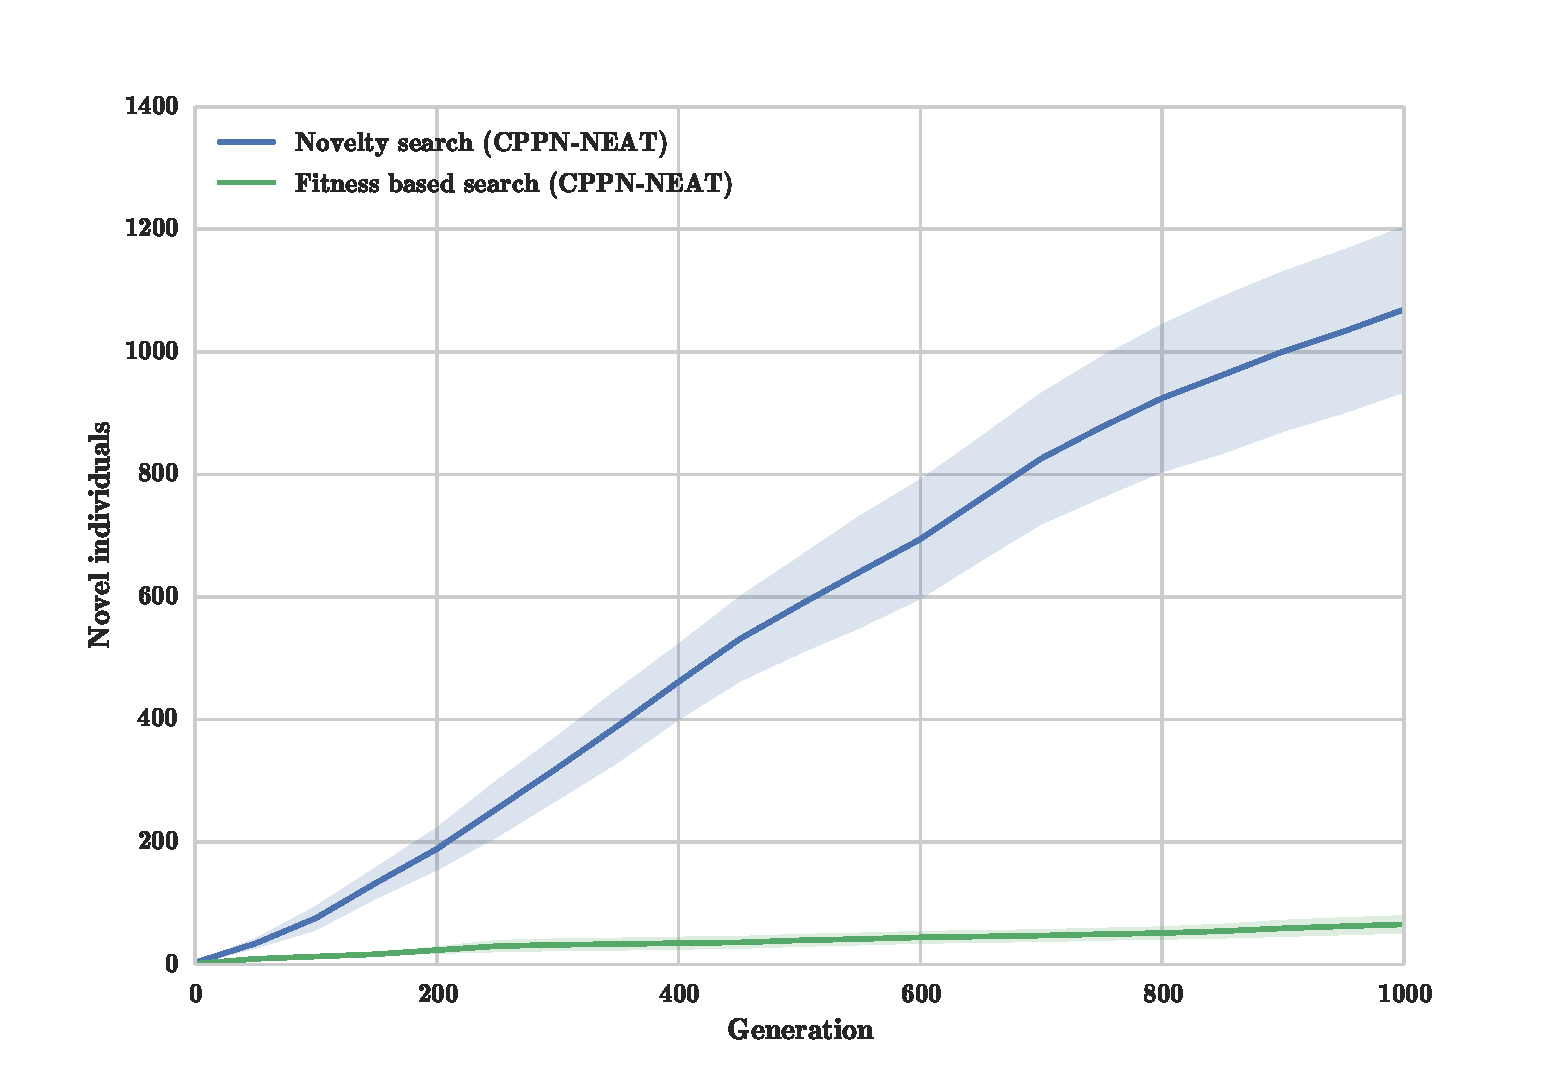
\includegraphics[width=1.0\textwidth]{Figures/Results/novelIndividualsFitNovComp.pdf}
\caption{Novel individual's behaviors upto generation averaged over 10 runs. The novelty is computed as the average distance from the $10$-nearest behaviors. The gravity acceleration for this experiment used was $-27.468\   m/s^2$, the size of the lattice $5\times 5\times5$ and $4$ available materials ($2$-actuated). Blue (Novelty search), Green (Fitness based search).}
\label{fig:ViolinPlotsAvgGenFitSize5}
\end{figure}



\begin{figure}
\centering
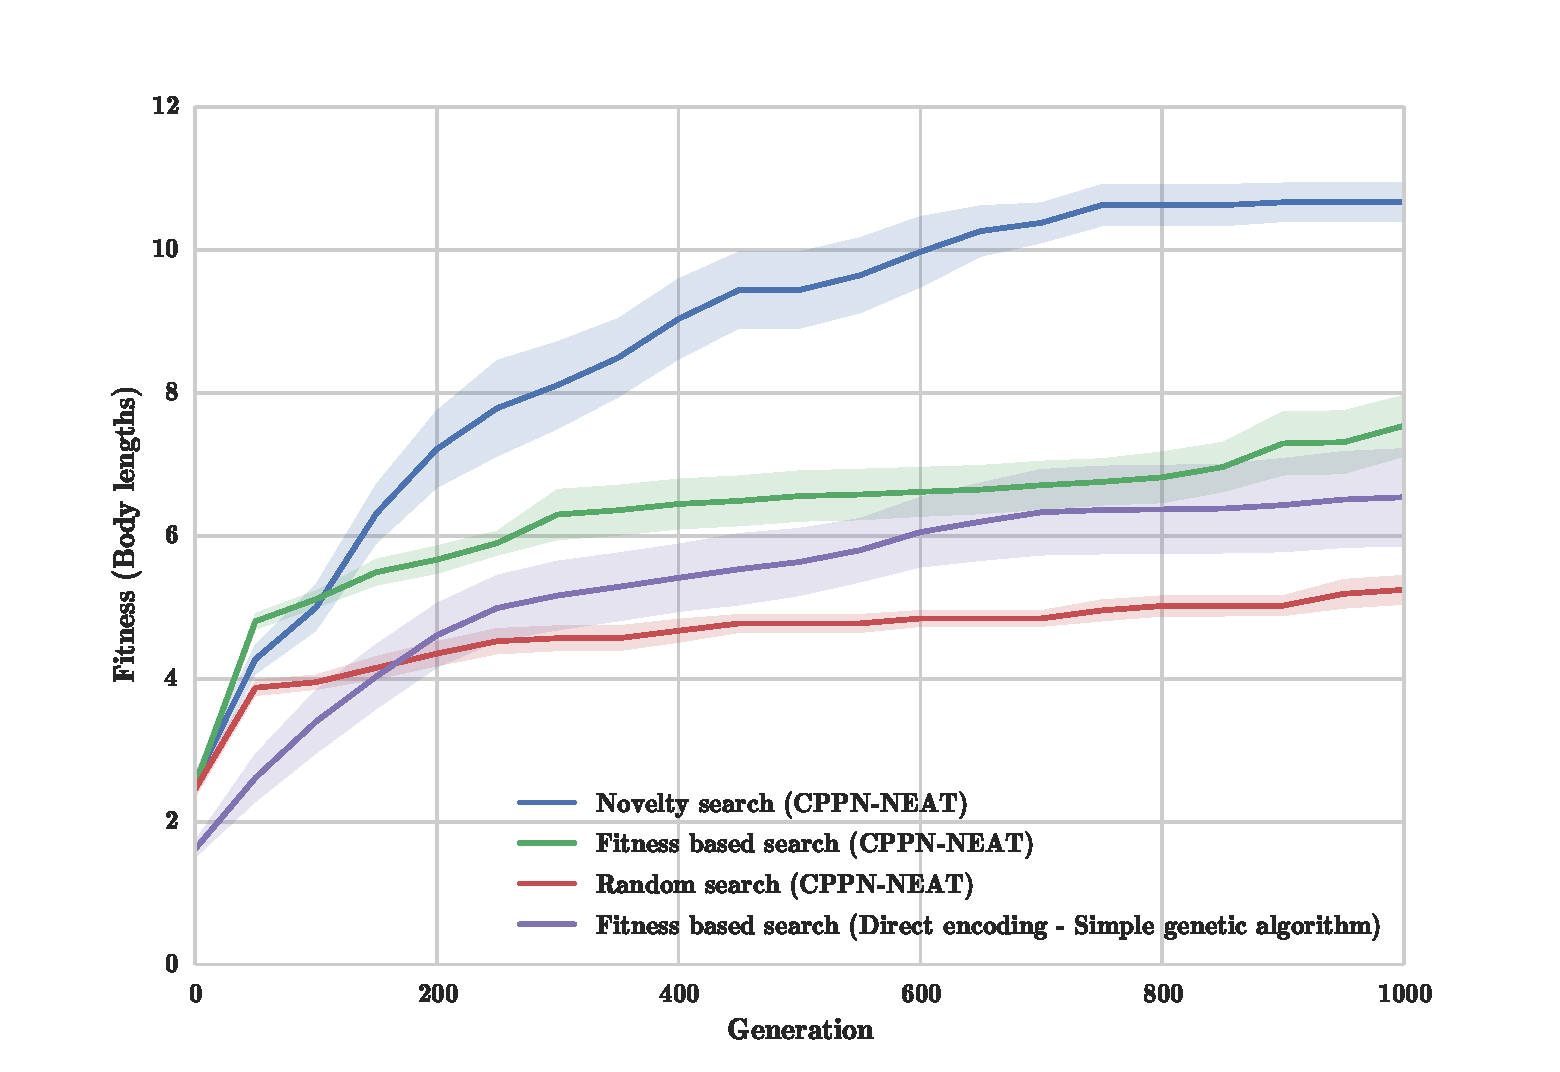
\includegraphics[width=1.0\textwidth]{Figures/Results/FitNovRandomDirectSize5.pdf}
\caption{Best so far fitness in body lengths displacement of softbot's center of mass averaged over $10$ runs together with the standard deviation error. The gravity acceleration for this experiment used was $-27.468\   m/s^2$, the size of the lattice $5\times 5\times5$ and $4$ available materials ($2$-actuated).}
\label{fig:FitNovRandomDirectSize5}
\end{figure}

\begin{figure}
\centering
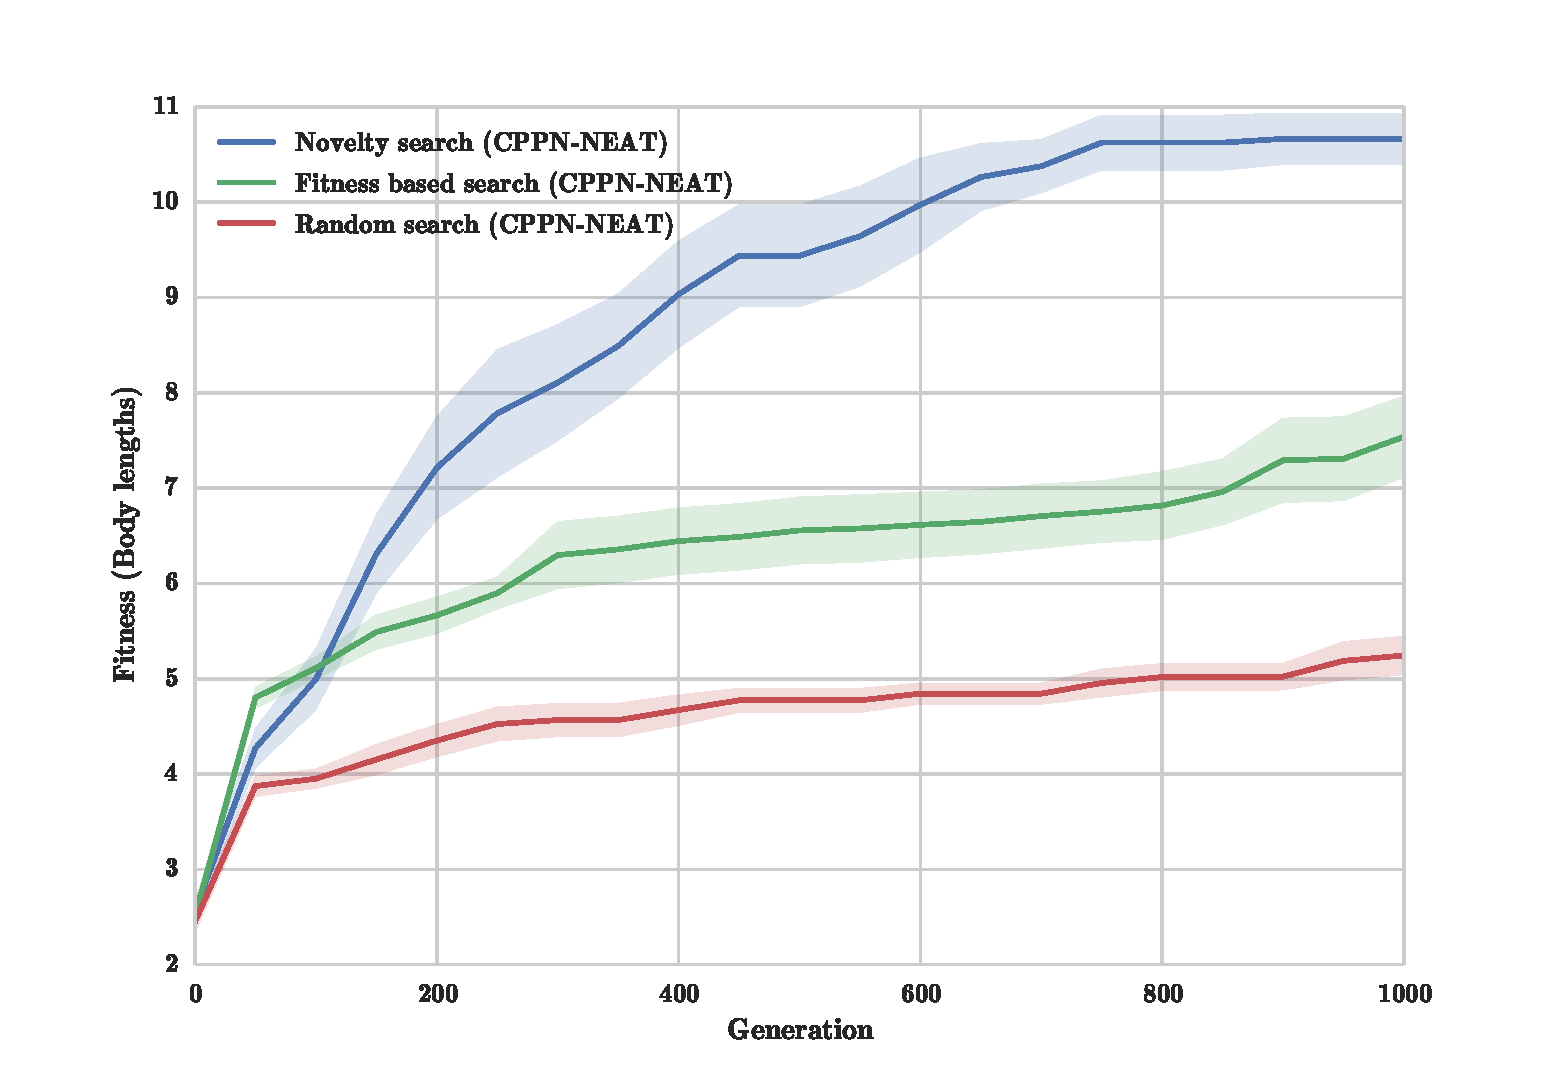
\includegraphics[width=1.0\textwidth]{Figures/Results/FitNovRandomSize5.pdf}
\caption{Best so far fitness in body lengths displacement of softbot's center of mass averaged over $10$ runs together with the standard deviation error. The gravity acceleration for this experiment used was $-27.468\   m/s^2$, the size of the lattice $5\times 5\times5$ and $4$ available materials ($2$-actuated).}
\label{fig:FitNovRandomSize5}
\end{figure}


\begin{figure}
\centering
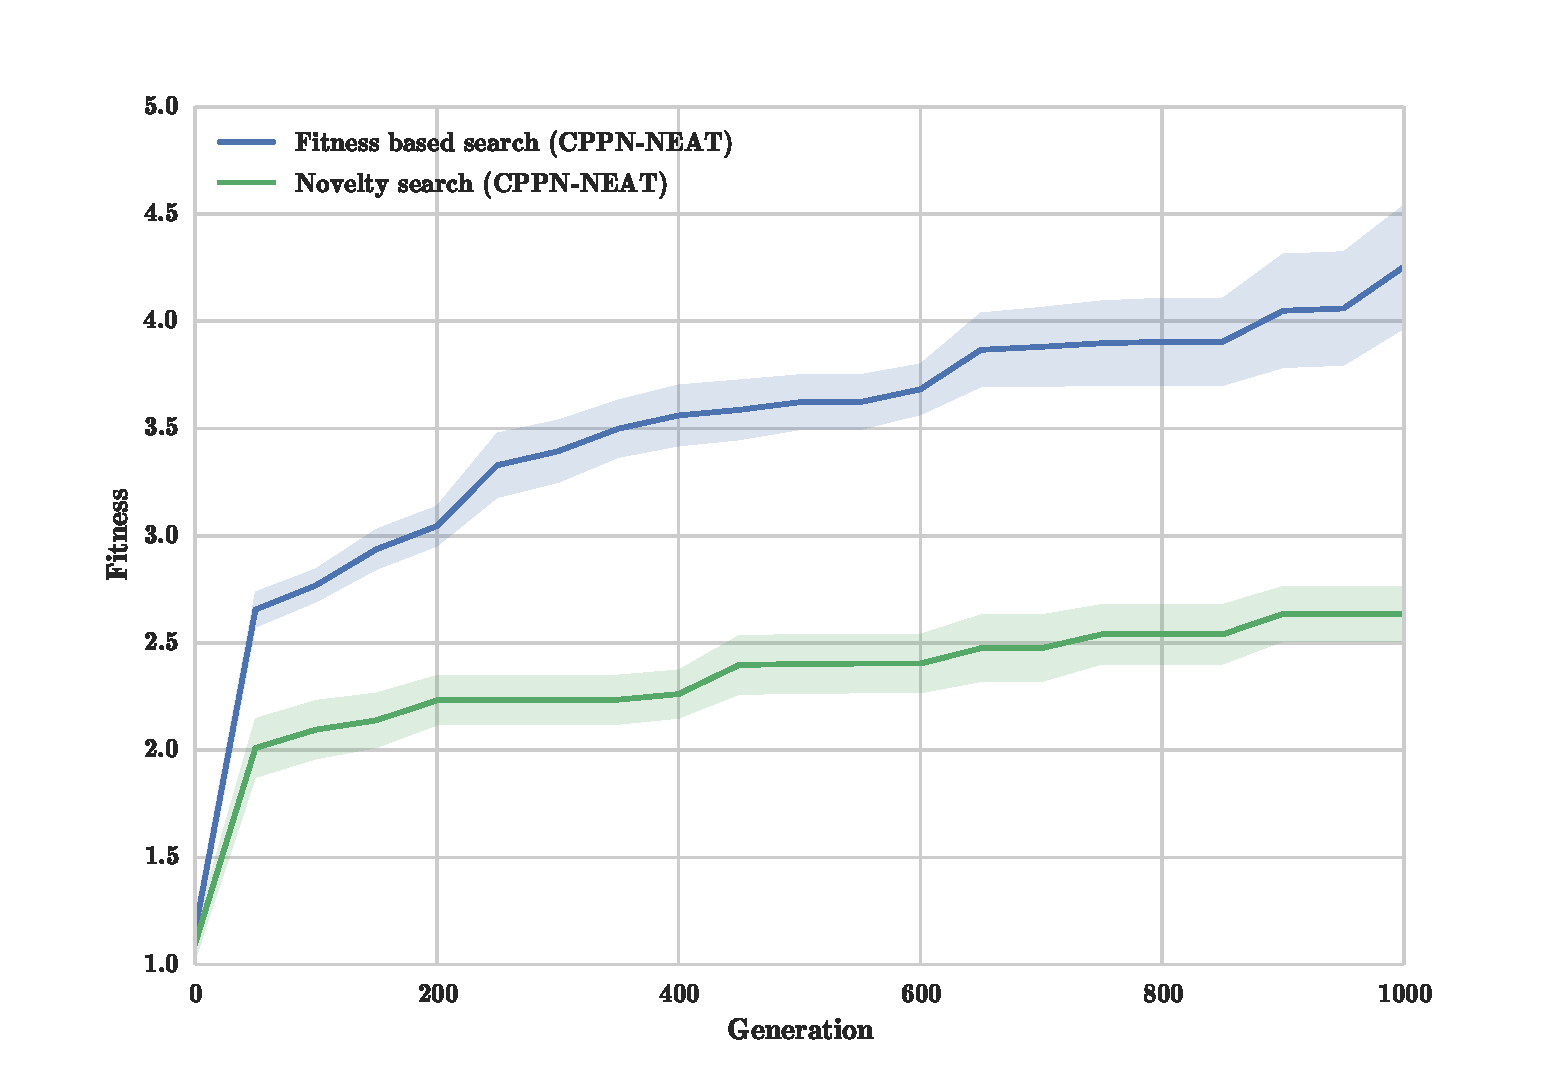
\includegraphics[width=1.0\textwidth]{Figures/Results/FitNovSize5Pen2.pdf}
\caption[]{Best so far fitness averaged over $10$ runs together with the standard deviation error penalizing actuated materials\footnotemark. The gravity acceleration for this experiment used was $-27.468\   m/s^2$, the size of the lattice $5\times 5\times5$ and $4$ available materials ($2$-actuated).}
\label{fig:FitNovRandomSize5}
\end{figure}

\footnotetext{Actuated materials penalize fitness: \[f = (1 - (n_{actuated} / n_{total})^{1.5}) \times disp \], where $n_{actuated}$, is the number of actuated voxels, $n_{total}$ total number of voxels and $disp$ the displacement of the softbot's center of mass.}












\clearpage
\subsection{Local competition in fitness based evolution}

\begin{figure}[h!]
\centering
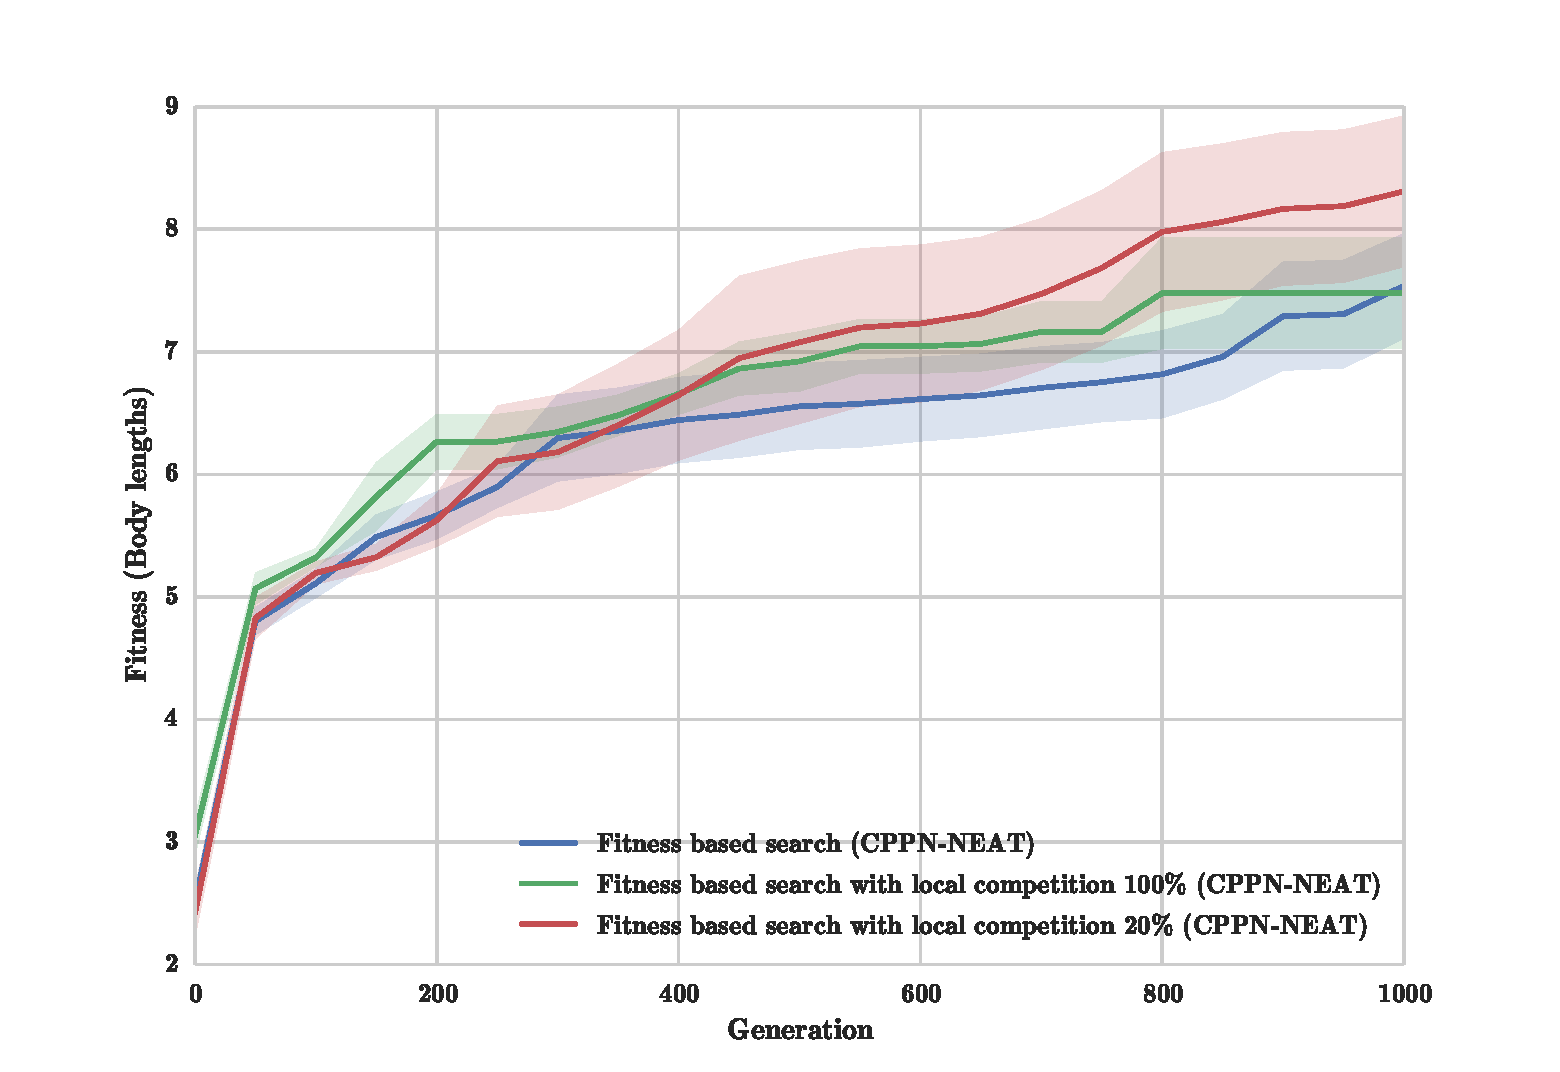
\includegraphics[width=1.0\textwidth]{Figures/Results/fitComp100_20percent.pdf}
\caption{Best so far fitness in body lengths displacement of softbot's center of mass averaged over $10$ runs together with the standard deviation error. Local competition is held among the top $20\%$ and in the complete population of each species. The gravity acceleration for this experiment used was $-27.468\   m/s^2$, the size of the lattice $5\times 5\times5$ and $4$ available materials ($2$-actuated).}
\label{fig:fitComp100_20percent}
\end{figure}

\begin{figure}[h!]
\centering
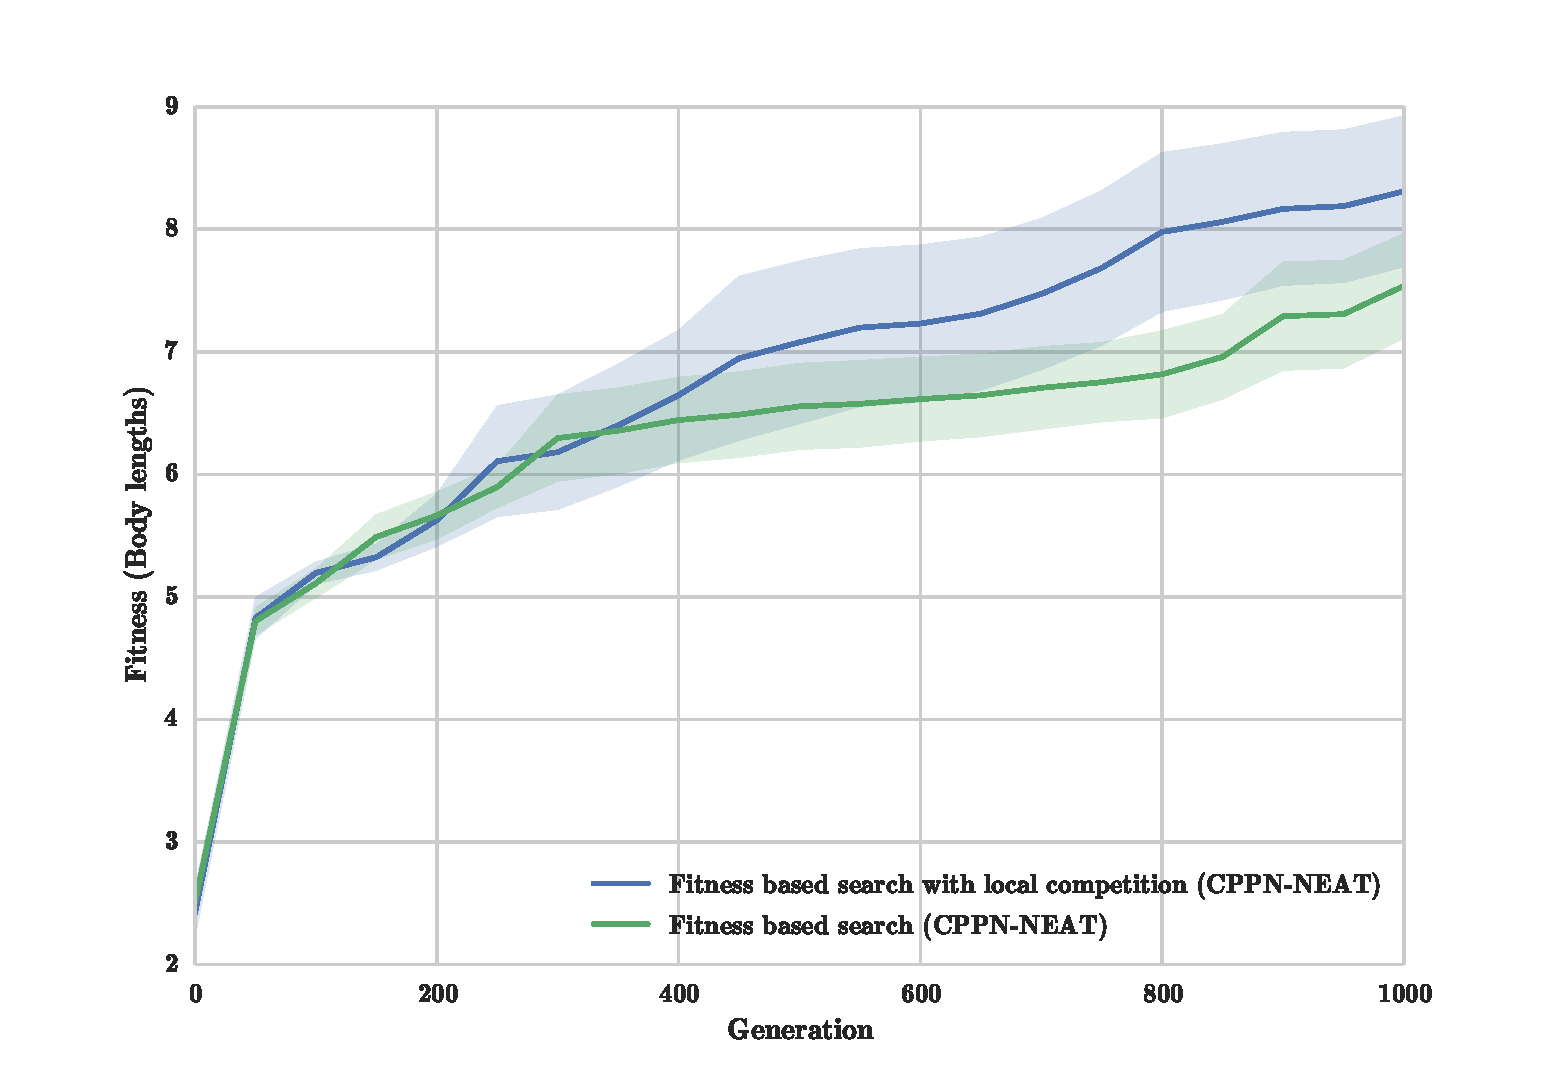
\includegraphics[width=1.0\textwidth]{Figures/Results/FitVsFitCompSize5.pdf}
\caption{Best so far fitness in body lengths displacement of softbot's center of mass averaged over $10$ runs together with the standard deviation error. Local competition is held among the top $20\%$ of each species population. The gravity acceleration for this experiment used was $-27.468\   m/s^2$, the size of the lattice $5\times 5\times5$ and $4$ available materials ($2$-actuated).}
\label{fig:FitVsFitCompSize5}
\end{figure}

\begin{figure}[h!]
\centering
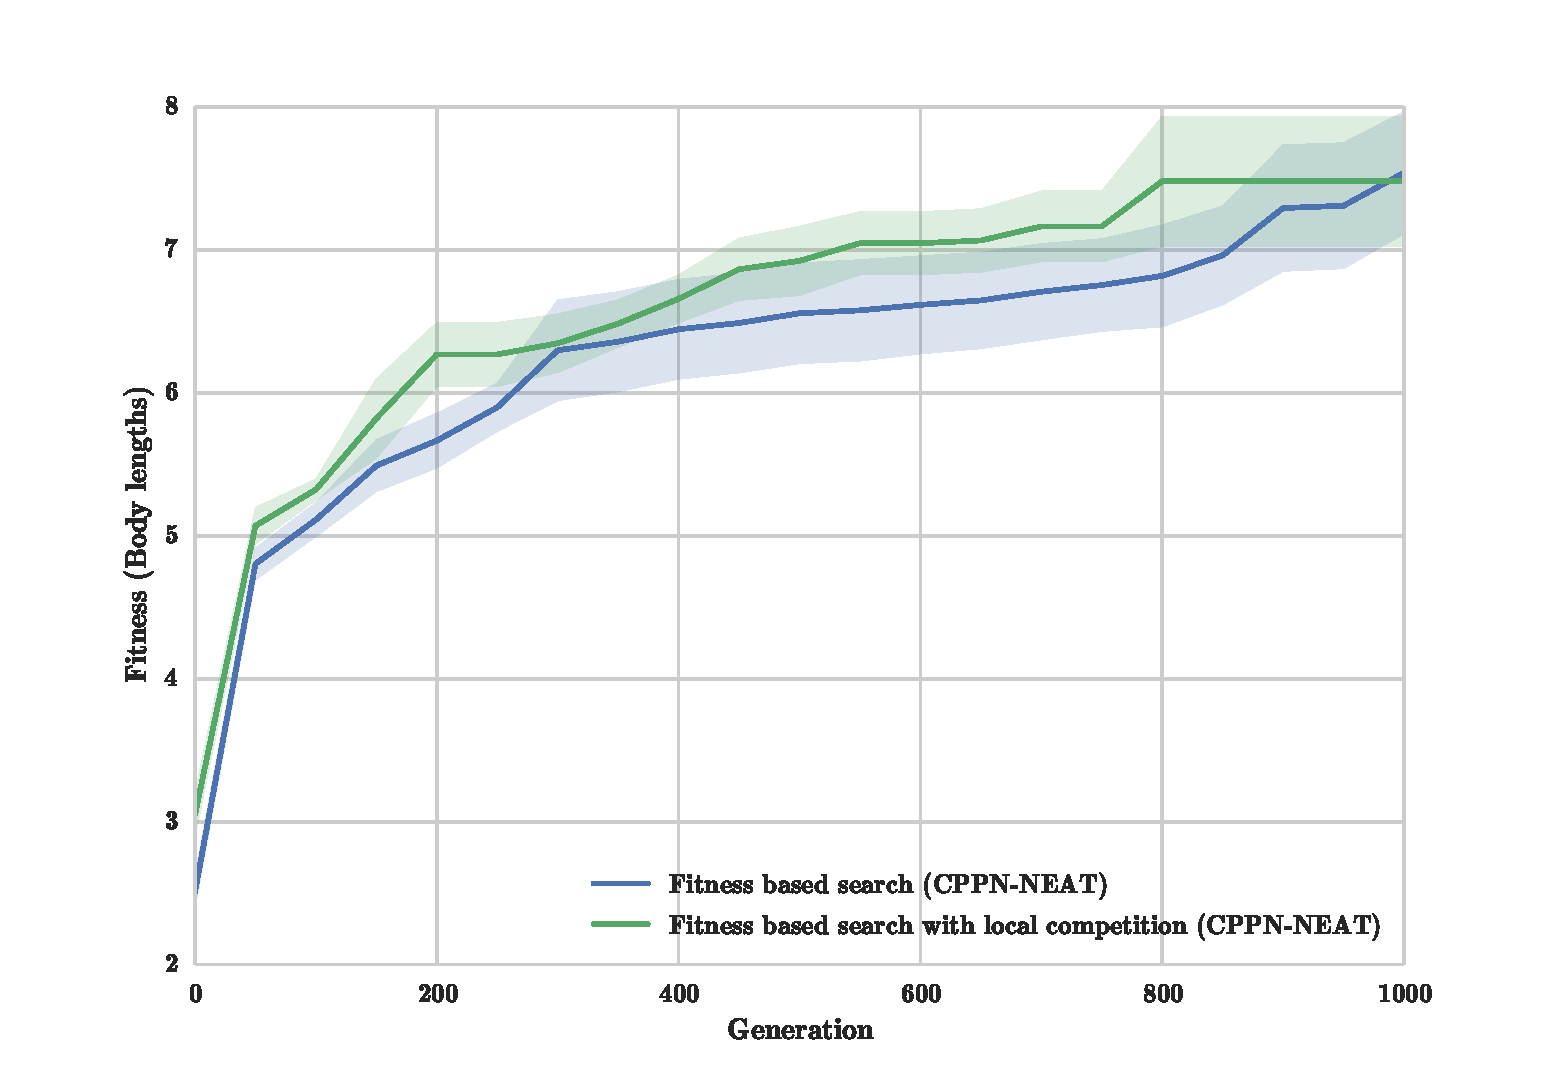
\includegraphics[width=1.0\textwidth]{Figures/Results/fitComp100percent.pdf}
\caption{Best so far fitness in body lengths displacement of softbot's center of mass averaged over $10$ runs together with the standard deviation error. Local competition is held among the complete population of each species. The gravity acceleration for this experiment used was $-27.468\   m/s^2$, the size of the lattice $5\times 5\times5$ and $4$ available materials ($2$-actuated).}
\label{fig:fitComp100percent}
\end{figure}










\clearpage
\subsection{Local competition in novelty search evolution}

\begin{figure}[h!]
{\centering
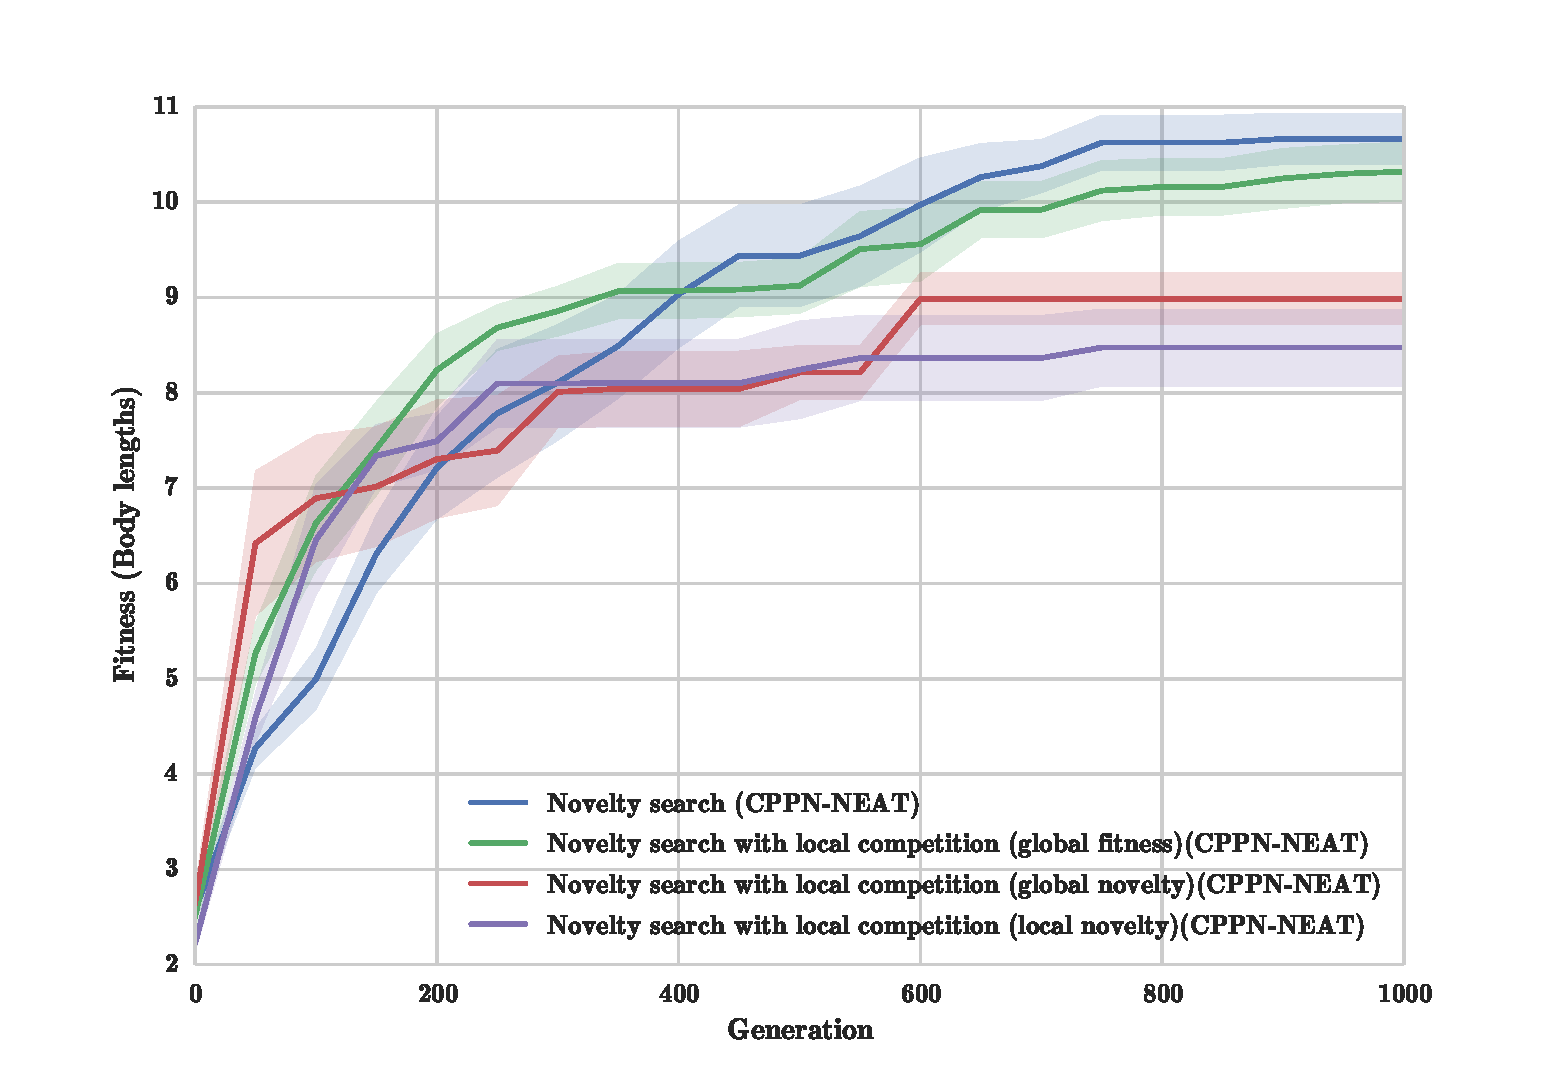
\includegraphics[width=1.0\textwidth]{Figures/Results/NoveltyCompetitionsSize5.pdf}}
\caption{Best so far fitness in body lengths displacement of softbot's center of mass averaged over $10$ runs together with the standard deviation error. Local competition is held among the complete population of each species. The gravity acceleration for this experiment used was $-27.468\   m/s^2$, the size of the lattice $5\times 5\times5$ and $4$ available materials ($2$-actuated).}
\label{fig:NoveltyCompetitionsSize5}
\end{figure}